\chapter{Vector Operator}
\section{Nabla Operator}

Ký hiệu Nabla, biểu diễn dưới dạng $\nabla$, là toán tử vi phân vector trong giải tích vector. 
Nó có thể đại diện cho các phép toán như gradient, divergence và curl.

\begin{enumerate}

\item \textit{Gradient.}

Cho đại lượng vô hướng $T(x,y,z)$, khi đó gradient của $T$ được biểu diễn:

\[
\nabla T
=
\frac{\partial T}{\partial x}\hat{x}
+
\frac{\partial T}{\partial y}\hat{y}
+
\frac{\partial T}{\partial z}\hat{z}.
\]

$\nabla T$ là một vector chỉ hướng tăng nhanh nhất của hàm $T$.

\textbf{Ví dụ:} Nếu nhiệt độ trong phòng thay đổi theo mọi hướng thì gradient chỉ hướng nhiệt độ tăng nhanh nhất.

\item \textit{Divergence.}

Divergence của vector $\mathbf{V}$ là phép nhân vô hướng giữa $\nabla$ và $\mathbf{V}$:

\[
\nabla \cdot \mathbf{V}
=
\frac{\partial v_x}{\partial x}
+
\frac{\partial v_y}{\partial y}
+
\frac{\partial v_z}{\partial z}.
\]

Divergence là một đại lượng vô hướng biểu thị độ phân tán của trường vector.

\item \textit{Curl.}

Curl của $\mathbf{V}$ là phép nhân có hướng giữa $\nabla$ và $\mathbf{V}$:

\[
\nabla \times \mathbf{V}
=
\begin{vmatrix}
\hat{x} & \hat{y} & \hat{z} \\
\frac{\partial}{\partial x} &
\frac{\partial}{\partial y} &
\frac{\partial}{\partial z} \\
v_x & v_y & v_z
\end{vmatrix}.
\]

Hay viết tường minh:

\[
\nabla \times \mathbf{V}
=
\left(
\frac{\partial v_z}{\partial y}
-
\frac{\partial v_y}{\partial z}
\right)\hat{x}
+
\left(
\frac{\partial v_x}{\partial z}
-
\frac{\partial v_z}{\partial x}
\right)\hat{y}
+
\left(
\frac{\partial v_y}{\partial x}
-
\frac{\partial v_x}{\partial y}
\right)\hat{z}.
\]

Curl đo mức độ xoáy cục bộ của trường vector.

\end{enumerate}
\section{Intergral Caculus}

\begin{enumerate}
    \item \textit{Line, Surface, and Volume Intergrals.}\\
    Trong giải tích nhiều biến và vật lý toán, khi hệ không còn gói gọn trên một trục số mà trải ra trong không gian, ta cần những công cụ tích phân vượt khỏi khuôn khổ “diện tích dưới đồ thị”.
Line integral, surface integral và volume integral chính là ba lớp công cụ cốt lõi để đo lường, tổng hợp và diễn giải các đại lượng phân bố theo đường, mặt, khối trong không gian.
\\
\begin{enumerate}[label=(\roman*)]
    \item \textbf{Line intergral}: đo độ dài tích lũy dọc theo quỹ đạo chuyển động.\\
    \item \textbf{Surface intergral}: đo mật độ hoặc dòng chảy (Flux) xuyên qua mặt định hướng.\\
    \item \textbf{Volume intergral}: đo mật độ hoặc số lượng nguồn nước bên trong khối.
\end{enumerate}

    \item \textit{Line intergral.}\\
    Nếu lấy tích phân theo một đường định hướng $\mathbf{P}$ bất kì từ vị trí đầu là $a$ và vị trí cuối là $b$ ta được công thức:
\[
    \int_{a\mathbf{P}}^{b} \mathbf{v} \cdot d\mathbf{I}
\]\\
    Mặt khác nếu đường đi của chúng ta là một vòng khép kín $\mathbf{C}$ tức là $a$ trùng với $b$ thì công thức sẽ là.
\[
    \oint_{C} \mathbf{v} \cdot d\mathbf{I}
\]\\
\textbf{example}: Một trong những ví dụng điển hình về tích phân trên trong vật lý đó là công thức tính công (\textbf{Work}) $\mathbf{W} = \mathbf{F} \cdot \ell$
\\
\item \textit{Surface intergral.}\\
Tương tự như \textbf{Line intergral} thì \textbf{Surface intergarl} cũng có hai dạng công thức đối với mặt định hướng thông thường và mặt đóng (ballon).
Trước hết ta cần định nghĩa vài công thức\\

\begin{enumerate}
  \item[(a)] Ta nói mặt định hướng là ám chỉ \textbf{mặt hai phía} trong giải tích hai.
  \item[(b)] ký hiệu $d \mathbf{a}$ trong sách ám chỉ mặt vi phân $\mathbf{a}$, là mặt định siêu nhỏ.
\end{enumerate}

Công thức \textbf{Surface itergral} đối với mặt định hướng thông thường.
\[
\int_{S} \mathbf{v} \cdot d\mathbf{a}
\]
\\
Công thức \textbf{Surface intergral} đối với mặt kín.
\[
\oint_{S} \mathbf{v} \cdot d\mathbf{a}
\]

\item \textit{Volume intergral.}\\
Khi một đại lượng không còn phân bố trên đường hay trên mặt, mà lan tỏa trong toàn bộ một miền không gian, ta cần đến \textbf{Volume intergarl} (tích phân trên khối) để mô tả tổng ảnh hưởng của nó.
\\ \\
\textbf{Volume intergral} là công cụ trung tâm để tổng hợp các đại lượng cục bộ thành một đại lượng toàn cục trong không gian ba chiều.
\[
\oint_{v} \mathbf{T} d\mathbf{\tau}
\]
\\ Trong đó:
\end{enumerate}
\begin{enumerate}
  \item[(a)] Ta lấy $\mathbf{T}$ là một hàm vô hướng (scalar function).
  \item[(b)] $\mathbf{d \tau}$ là phần tử vi phân thể tích không có hướng.
\end{enumerate}

\section{Special Coordinates}

\begin{enumerate}
\item \textit{Curvilinear Coordinates}\\
    Tọa độ cầu trong vật lý không chỉ là đổi hệ trục cho “đẹp”. Nó là cách tự nhiên nhất để mô tả những hệ có \textbf{đối xứng xuyên tâm}. Khi bài toán không phân biệt hướng ngang dọc mà chỉ quan tâm khoảng cách xa gần tính từ gốc.
\begin{figure}[htbp]
    \centering
    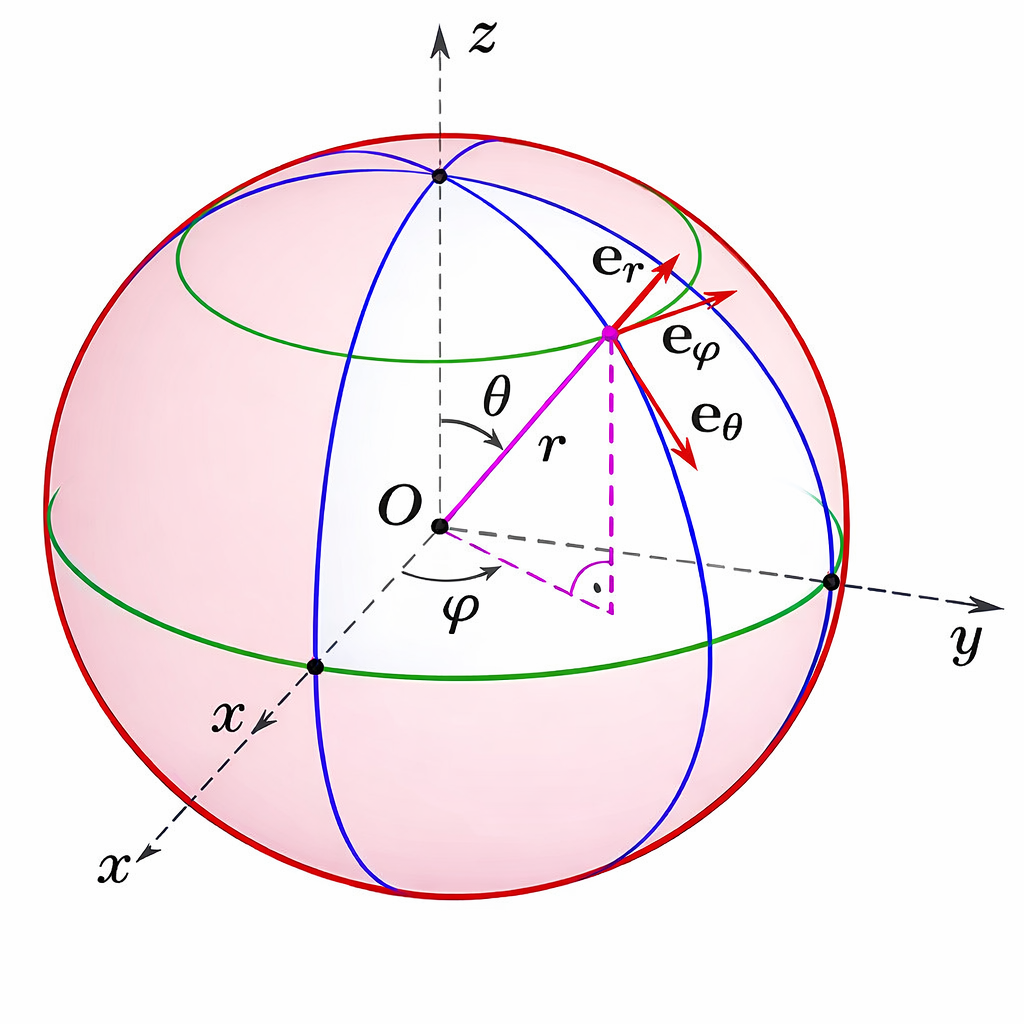
\includegraphics[width=0.6\textwidth]{Toa_Do_Cau.png}
    \label{fig:p1}
\end{figure}\\
   Cho Vector $\mathbf{v} =(x\hat{x}+y\hat{y}+z\hat{z})$ sẽ được biễu diễn trong tọa độ cầu như sau:
\[
\mathbf{v}=
\begin{bmatrix}
x\\
y\\
z
\end{bmatrix}
=
\begin{bmatrix}
r\sin\theta\cos\phi\\
r\sin\theta\sin\phi\\
r\cos\theta
\end{bmatrix}
\]

Ta cần tính $\hat{e}_{r}, \hat{e}_{\phi}, \hat{e}_{\theta}$.

\[
\hat{\theta}
=
\frac{1}{r}\frac{\partial \mathbf{v}}{\partial \theta}
=
\begin{bmatrix}
\cos\theta\cos\phi\\
\cos\theta\sin\phi\\
-\sin\theta
\end{bmatrix}
\]

\[
\hat{\phi}
=
\frac{1}{r\sin\theta}\frac{\partial \mathbf{v}}{\partial \phi}
=
\begin{bmatrix}
-\sin\phi\\
\cos\phi\\
0
\end{bmatrix}
\]

\[
\hat{r}
=
\frac{\partial \mathbf{v}}{\partial r}
=
\begin{bmatrix}
\sin\theta\cos\phi\\
\sin\theta\sin\phi\\
\cos\theta
\end{bmatrix}
\]

Lấy chuẩn ta được:

\[
\begin{cases}
\hat{\theta} =
\cos\theta\cos\phi\,\hat{x}+
\cos\theta\sin\phi\,\hat{y}-
\sin\theta\,\hat{z}\\[6pt]

\hat{\phi} =
-\sin\phi\,\hat{x}+
\cos\phi\,\hat{y}\\[6pt]

\hat{r} =
\sin\theta\cos\phi\,\hat{x}+
\sin\theta\sin\phi\,\hat{y}+
\cos\theta\,\hat{z}
\end{cases}
\]

\[
\nabla
=
\hat{\mathbf e}_r\,\frac{\partial}{\partial r}
+\hat{\mathbf e}_\theta\,\frac{1}{r}\frac{\partial}{\partial \theta}
+\hat{\mathbf e}_\phi\,\frac{1}{r\sin\theta}\frac{\partial}{\partial \phi}
\]

\[
\nabla f
=
\hat{\mathbf e}_r\,\frac{\partial f}{\partial r}
+\hat{\mathbf e}_\theta\,\frac{1}{r}\frac{\partial f}{\partial \theta}
+\hat{\mathbf e}_\phi\,\frac{1}{r\sin\theta}\frac{\partial f}{\partial \phi}
\]

\[
\nabla\cdot \mathbf A
=
\frac{1}{r^2}\frac{\partial}{\partial r}\left(r^2 A_r\right)
+\frac{1}{r\sin\theta}\frac{\partial}{\partial \theta}\left(\sin\theta A_\theta\right)
+\frac{1}{r\sin\theta}\frac{\partial A_\phi}{\partial \phi}
\]

$
\nabla\times \mathbf A
=
\left[
\frac{1}{r\sin\theta}
\left(
\frac{\partial}{\partial \theta}(\sin\theta A_\phi)
-
\frac{\partial A_\theta}{\partial \phi}
\right)
\right]\hat{\mathbf e}_r
+
\left[
\frac{1}{r}
\left(
\frac{1}{\sin\theta}\frac{\partial A_r}{\partial \phi}
-
\frac{\partial}{\partial r}(rA_\phi)
\right)
\right]\hat{\mathbf e}_\theta
+
\left[
\frac{1}{r}
\left(
\frac{\partial}{\partial r}(rA_\theta)
-
\frac{\partial A_r}{\partial \theta}
\right)
\right]\hat{\mathbf e}_\phi
$
\end{enumerate}

\section{The theory of vector field.}
\begin{enumerate}

\item \textit{The Helmholtz theorem.}

Trong vật lý có một câu hỏi rất cơ bản: một trường vector được xác định bởi những thông tin cơ bản nào? 
Cụ thể nếu ta biết $\nabla \cdot F$ và $\nabla \times F$ thì liệu có đủ để xác định hoàn toàn trường đó hay không?

Chẳng hạn ta biết trước hàm vô hướng $D$ thỏa mãn
\[
\nabla \cdot F = D
\]
và trường vector $C$ thỏa
\[
\nabla \times F = C.
\]

Câu trả lời là chưa hẳn. Ví dụ tồn tại những trường đặc biệt có cả $\nabla \cdot F = 0$ và $\nabla \times F = 0$ ở mọi nơi như $F = yz\hat{x} + xz\hat{y} + zy\hat{z}$ , $F = \sin{x}\cosh{y}\hat{x} - \cos{x}\sinh{y}\hat{y}$...
Tuy nhiên khi giải phương trình vi phân ta cần cung cấp điều kiện biên để nghiệm là duy nhất, điều đó giúp ta tìm được chính xác hàm ta muốn.

Trong điện từ học, ta yêu cầu trường tiến về $0$ ở vô cực. Khi đó định lý Helmholtz đảm bảo rằng trường được xác định duy nhất bởi $\nabla \cdot F$ và $\nabla \times F$

Cho F là một trường vector được xác định trên không gian, thỏa các điều kiện suy giảm thích hợp ở vô cực, khi đó F có thể xác định bởi trường vô hướng $\phi$ và trường vector $A$ như sau,
\[
F = -\nabla \phi + \nabla \times A.
\]

\item \textit{Potentials.}

Nếu $\nabla \times F = 0$ thì tồn tại hàm thế vô hướng $V$ sao cho
\[
F = -\nabla V.
\]

\textbf{Định lý 1 (Irrotational fields).} Các mệnh đề sau tương đương:

\begin{enumerate}
\item[(a)] $\nabla \times F = 0$
\item[(b)] $\displaystyle \int_a^b F \cdot dl$ không phụ thuộc đường đi
\item[(c)] $\displaystyle \oint F \cdot dl = 0$
\item[(d)] $F = -\nabla V$
\end{enumerate}

Hàm thế không duy nhất vì $V$ có thể thay bằng $V+c$.

Nếu $\nabla \cdot F = 0$ thì tồn tại vector thế $A$ sao cho
\[
F = \nabla \times A.
\]

\textbf{Định lý 2 (Solenoidal fields).} Các mệnh đề sau tương đương:

\begin{enumerate}
\item[(a)] $\nabla \cdot F = 0$
\item[(b)] $\displaystyle \int F \cdot da$ không phụ thuộc mặt
\item[(c)] $\displaystyle \oint F \cdot da = 0$
\item[(d)] $F = \nabla \times A$
\end{enumerate}

Vector thế không duy nhất vì
\[
\nabla \times A = \nabla \times (A + \nabla \lambda).
\]

\end{enumerate}